\section{Phase 1 Results: Features and Graph WaveNet}
\label{sec:results}
The full test-set comparison of all models, Phase~1 and Phase~2, is in
Table~\ref{tab:p2main} (Section~\ref{sec:p2results}). Here we summarise the Phase~1
findings that shaped Phase~2.

\textbf{Features.} The cumulative ablation (Table~\ref{tab:feat_ablation},
Fig.~\ref{fig:fe}) shows that the weekly profile is the most valuable group at long
horizons: it cuts 60-minute validation MAE from 3.96 to 3.52\,mph. Calendar
features help at every horizon. Upstream and downstream aggregates still help
afterwards (3.52$\to$3.43 at 60\,min), which is the first evidence that neighbouring
segments carry information a segment's own history lacks. Permutation importance
agrees: at 15\,min the profile at the target time and the latest lag dominate, while
at 60\,min the profile dominates and the downstream anomaly is the third most
important feature.

\begin{table}[t]
\centering
\caption{Cumulative feature-group ablation for gradient boosting (validation MAE, mph).}
\label{tab:feat_ablation}
\begin{tabular}{lccc}
\toprule
Feature groups & 15 min & 30 min & 60 min \\
\midrule
lags & 2.832 & 3.423 & 4.360 \\
+window stats & 2.823 & 3.412 & 4.341 \\
+calendar & 2.756 & 3.256 & 3.962 \\
+weekly profile & 2.736 & 3.126 & 3.517 \\
+spatial & 2.684 & 3.052 & 3.432 \\
+sensor stats & 2.675 & 3.038 & 3.411 \\
\bottomrule
\end{tabular}
\end{table}

\begin{figure*}[t]
\centering
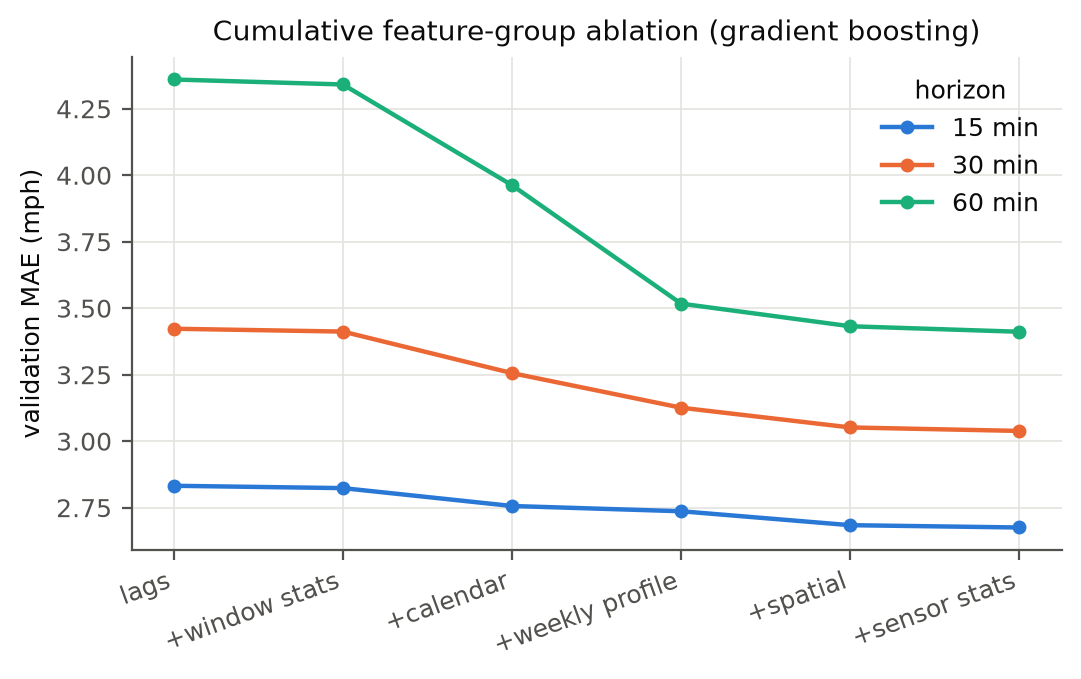
\includegraphics[width=0.42\textwidth]{fe_ablation.png}\hfill
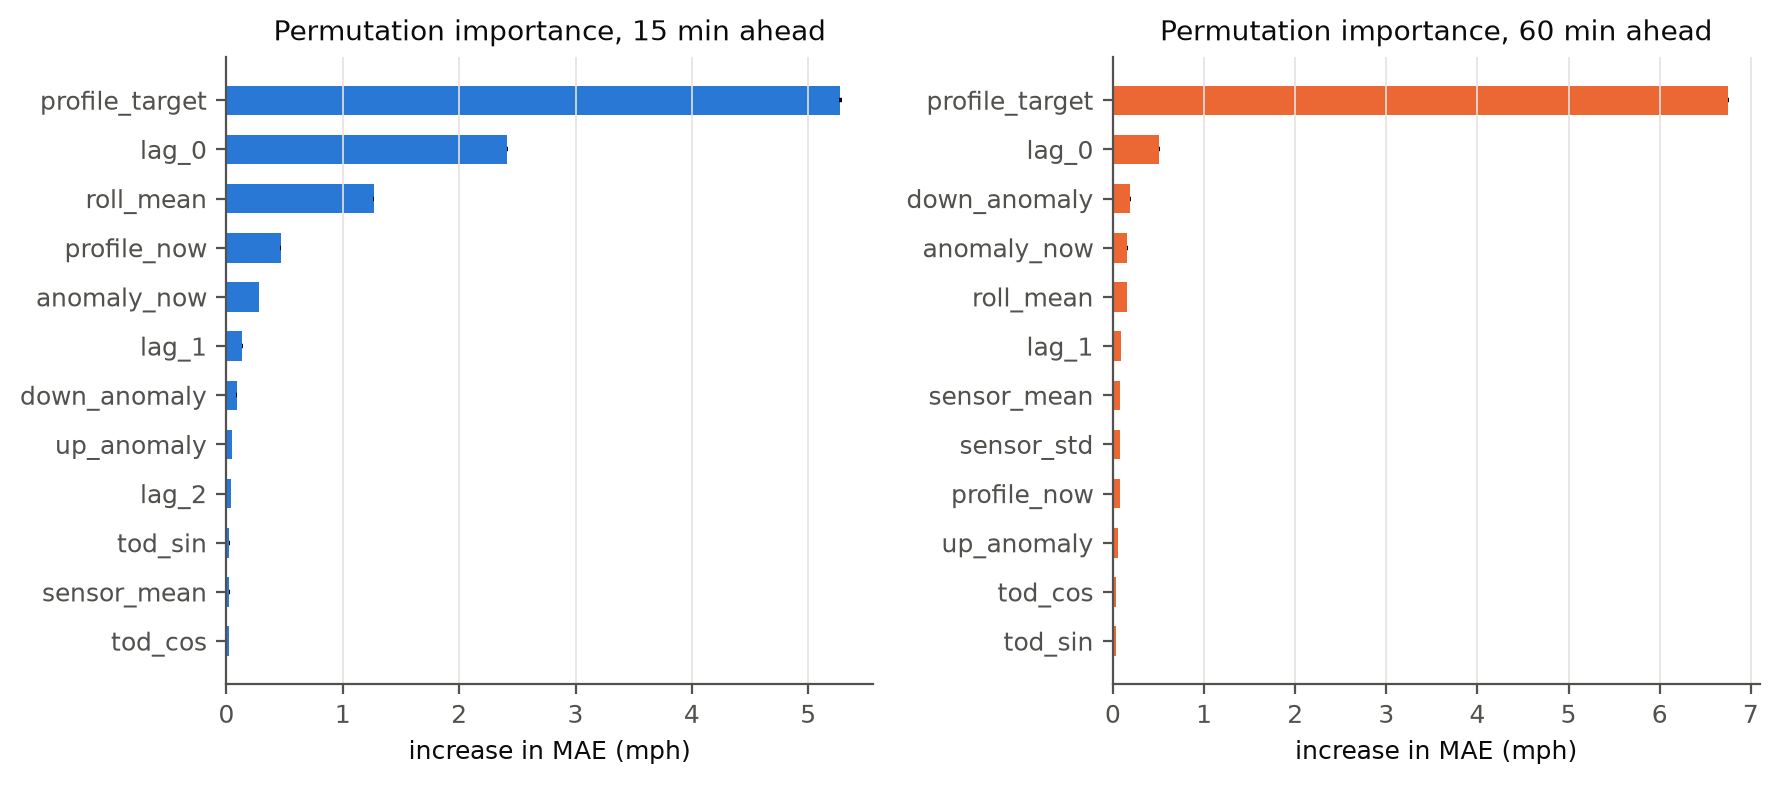
\includegraphics[width=0.55\textwidth]{fe_permutation_importance.png}
\caption{Left: cumulative feature-group ablation for gradient boosting. Right:
permutation importance at 15 and 60\,min (increase in validation MAE).}
\label{fig:fe}
\end{figure*}

\textbf{Graph WaveNet versus engineered features.} Graph WaveNet beats gradient
boosting at every horizon (2.72/3.10/3.59 vs.\ 2.89/3.29/3.66\,mph), and
Diebold--Mariano tests reject equal accuracy ($p<0.001$ at all horizons;
Table~\ref{tab:p2dm} contains the Phase~2 pairs). At 60\,min, however, the margin is
only 0.07\,mph, and gradient boosting trains in 10~minutes on a CPU against 2.4~hours
on a laptop GPU. Our Graph WaveNet reproduces the published
numbers closely (3.59 vs.\ 3.53\,mph at 60\,min) despite stopping after 26 epochs.

\textbf{What Graph WaveNet's learned graph learns.} The self-adaptive adjacency
is close to uniform: its mean row entropy is 5.23 against a maximum of
$\ln 207=5.33$, and its top-5 neighbours overlap the road graph \emph{less} than
random (lift 0.87; Fig.~\ref{fig:adj}). In our run it acts as a global mixing term
rather than discovering hidden links. This is one reason Phase~2 returns to the
fixed road graph and lets attention, rather than a free $N{\times}N$ matrix, decide
how much each real neighbour matters.

\begin{figure}[t]
\centering
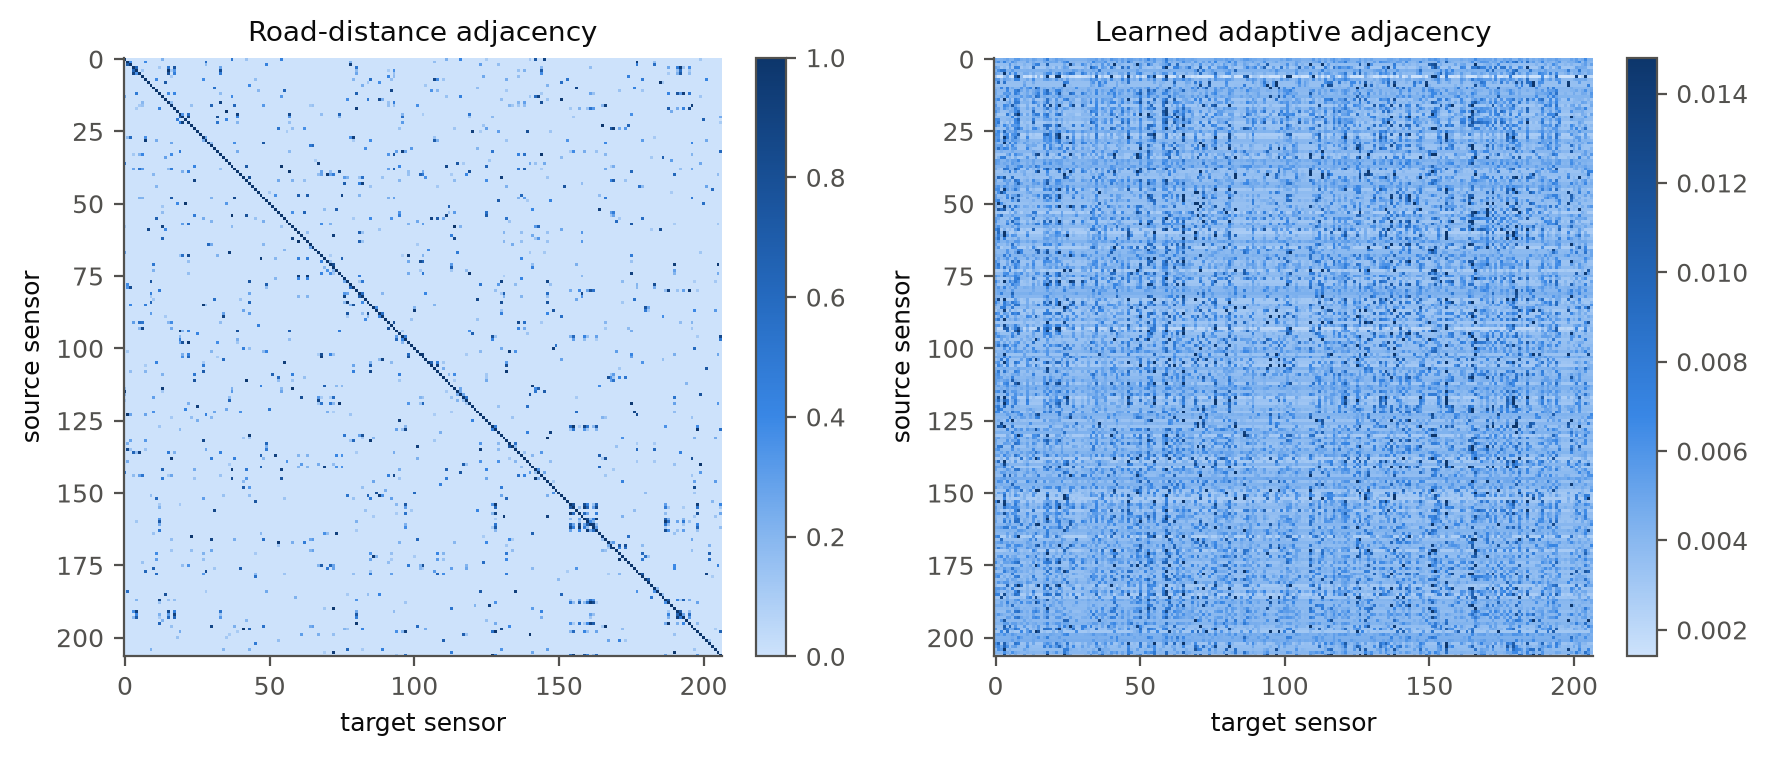
\includegraphics[width=\columnwidth]{res_adjacency.png}
\caption{Road-distance adjacency (left) and Graph WaveNet's learned adaptive
adjacency (right).}
\label{fig:adj}
\end{figure}

\textbf{When and where errors occur.} Error peaks at the evening rush
(Fig.~\ref{fig:hour}) and at a minority of sensors. Most strikingly, Graph WaveNet is
\emph{less robust to outages} than gradient boosting. When the latest input reading
is missing, its 60-minute MAE rises from 3.54 to 5.36\,mph (+52\,\%), against 3.63
to 4.50\,mph (+24\,\%) for gradient boosting, whose features are forward-filled. The
DCRNN-style pipeline shows the network an outage as a reading of 0\,mph.
This observation motivates the masked inputs of Section~\ref{sec:dldata}.

\begin{figure}[t]
\centering
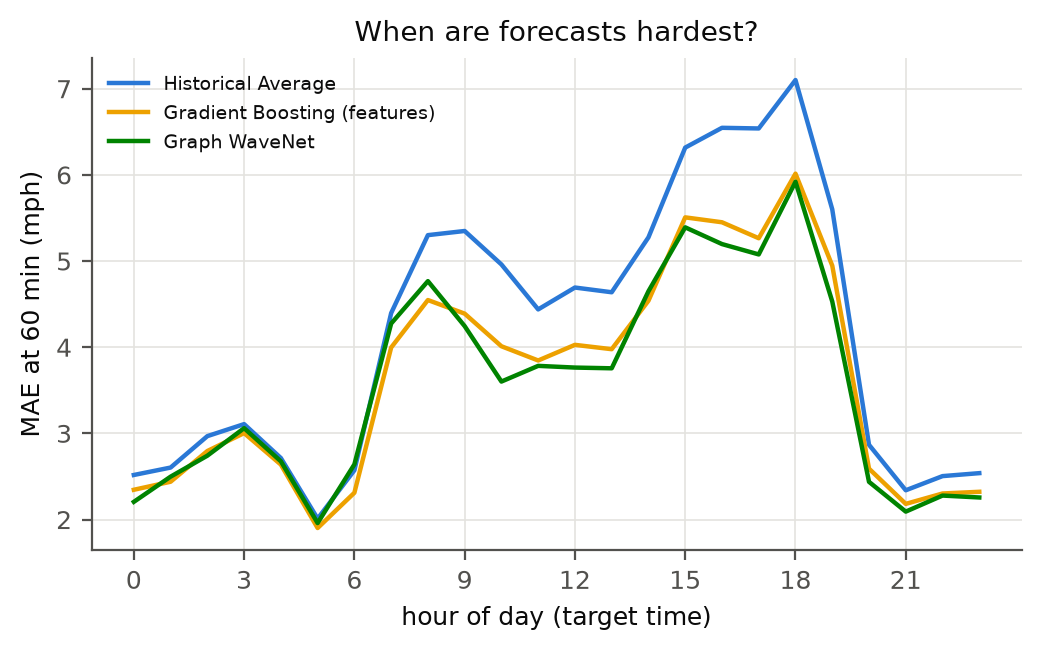
\includegraphics[width=\columnwidth]{res_mae_by_hour.png}
\caption{60-minute MAE by hour of the target time.}
\label{fig:hour}
\end{figure}
